\documentclass[a4paper,11pt]{article}

\usepackage[T1]{polski}
\usepackage[utf8]{inputenc} 
\usepackage{graphicx}
\usepackage{float}
\usepackage{verbatim}
\hoffset=-3.0cm                 % Mniejszy lewy margines
\textwidth=18cm                 % szerzej
\evensidemargin=0pt

\voffset=-3cm                   % Mniejszy gorny margines
\textheight=27cm                % szerzej wzdluz

\usepackage{listings}
% Listingi
\lstdefinestyle{customc}{
	belowcaptionskip=1\baselineskip,
	breaklines=true,
	frame=L,
	xleftmargin=0pt,
	language=HTML,
	showstringspaces=false,
	basicstyle=\footnotesize\ttfamily,
	identifierstyle=\color{black}
}

\setlength{\parindent}{0pt}             % No paragraph indentation
\setlength{\parskip}{\medskipamount}    % Space between paragraphs
\raggedbottom   


\title{POLITECHNIKA WARSZAWSKA \\ WYDZIAŁ ELEKTRYCZNY \\}
\author{Michał Sut}
\date{\today}

\begin{document}
	\thispagestyle{empty}
	\maketitle
	\date{}
	\section{Treść zadania}
	Napisać program umożliwiający znalezienie maksimum funkcji dopasowania jednej 
	zmiennej określonej dla liczb całkowitych w zadanym zakresie przy pomocy 
	elementarnego algorytmu genetycznego (reprodukcja z użyciem nieproporcjonalnej 
	ruletki, krzyżowanie proste, mutacja równomierna). Program powinien umożliwiać 
	użycie różnych funkcji dopasowania, populacji o różnej liczebności oraz różnych 
	parametrów operacji genetycznych (krzyżowania i mutacji). Program powinien 
	zapewnić wizualizację wyników w postaci wykresów średniego, maksymalnego 
	i minimalnego przystosowania dla kolejnych populacji oraz wykresu funkcji 
	w zadanym przedziale. 
	
	Program przetestować dla funkcji$ f(x)= -0.1x^2 + 4x + 7 $ dla $x= -1, 0, ... 41 $

	\section{Instrukcja działania programu}
		\subsection{Okno główne programu}
			\begin{figure}[H]
				\centering
				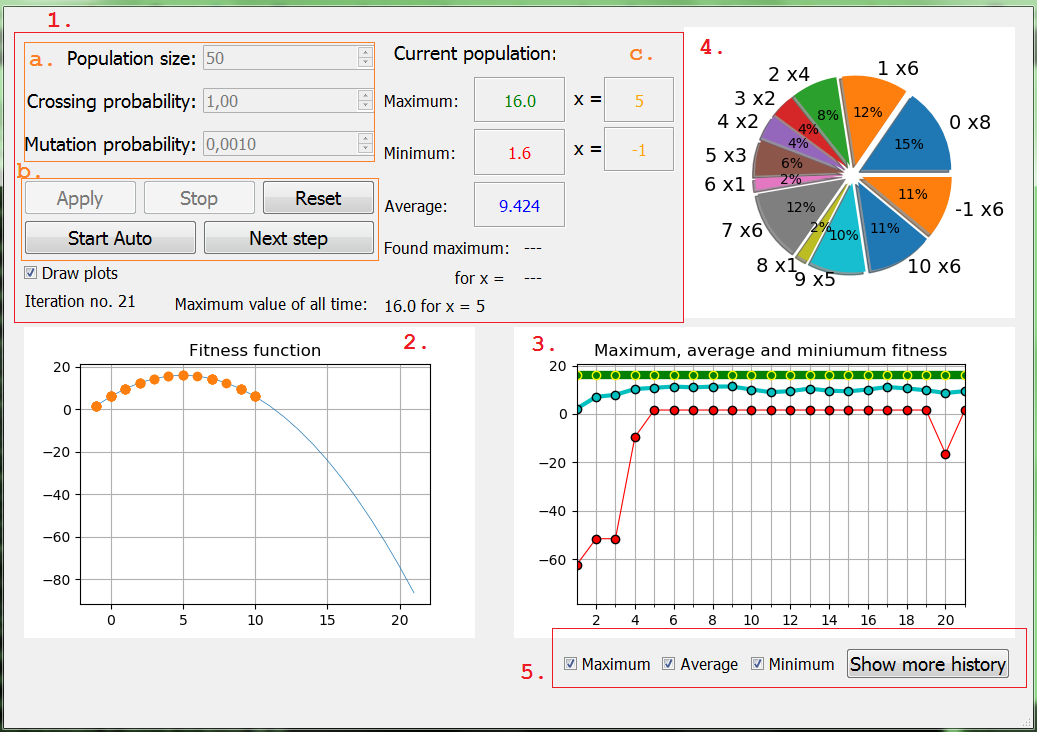
\includegraphics[scale=0.6]{main_window2.png}
			\end{figure}
		
		\subsection{Opis okna programu}
			\begin{enumerate}
				\item Panel sterowania
				\begin{enumerate}
					\item Parametry populacji
					\item Przyciski sterowania
					\item Wszystkie informacje gromadzone i wyliczone podczas działania programu
				\end{enumerate}
				\item Wykres funkcji z zaznaczonymi osobnikami populacji
				\item Wykres wartości średnich, maksymalnych i minimalnych dla kolejnych generacji. Pokazuje określoną liczbę ostatnich wyników. 
				\item Wykres kołowy przedstawiający "nieproporcjonalną ruletkę", czyli prawdopodobieństwo wylosowania danego osobnika
				\item Panel umożliwiający podejrzenie całego wykresu, aż od początkowej generacji.
			\end{enumerate}
		
		\subsection{Zmiana ustawień programu}
			Ustawienia programu znajdują się w pliku \texttt{settings.py}. Zmianą podlegają następujące elementy:
			\begin{enumerate}
				\item \textbf{FUNCTION} - Funkcja dopasowania
				\item \textbf{X\_START} - Początek zakresu
				\item \textbf{X\_END} - Koniec zakresu
				\item \textbf{MAX\_HIST\_SIZE} - Liczba wyników pokazywana na wykresie wartości min/max/avg
			\end{enumerate}
	
		\subsection{Użycie}
			\subsubsection{Podstawowe operacje}
				\begin{enumerate}
					\item Ustawić parametry populacji
					\item Zainicjować populację klikając przycisk \framebox{ \texttt{Apply}}
					\item W tym momencie dostępne są trzy możliwości:
					\begin{enumerate}
						\item \framebox{Next Step} - Wykonanie tylko jednej generacji
						\item \framebox{Start Auto} - Wykonywanie kolejnych generacji aż do wystąpienia warunku stopu
						\item \framebox{Reset} - Wyczyszczenie populacji i jej parametrów
					\end{enumerate}
					\item Rozpoczęty proces automatycznych generacji można zastopować przyciskiem \framebox{Stop}
				\end{enumerate}
				
				Zaznaczając lub odznaczając pole \texttt{Draw plots} decydujemy o tym, czy kolejne generacje będą wyświetlane na wykresach.\\
				\emph{Uwaga! Zaznaczenie pola powoduje wydłużenie czasu trwania wykonania jednego pełnego kroku. Ma to szczególne znaczenie podczas generacji automatycznych.}
			\subsubsection{Otworzenie pełnego wykresu wartości średnich, maksymalnych i minimalnych}
			Przycisk \framebox{Show more history} powoduje otworzenie nowego okna z pełnym wykresem wartości, które zostały zaznaczone w polach, znajdujących się obok przycisku. Nowo otwarte okno wygląda następująco: 
			\begin{figure}[H]
				\centering
				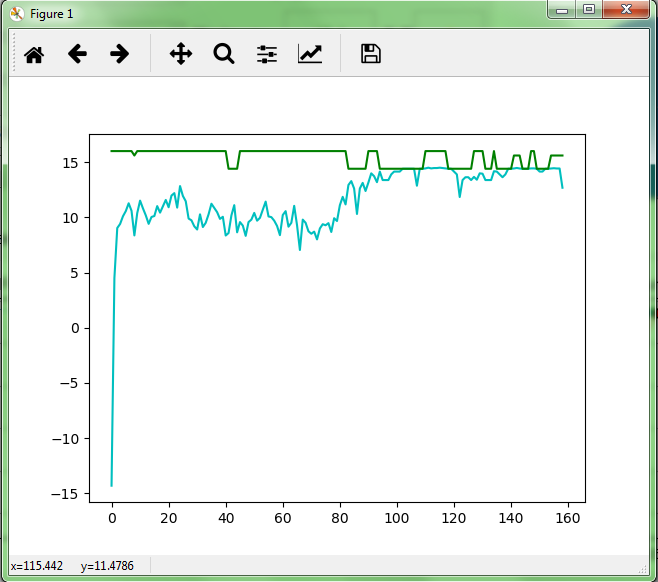
\includegraphics[scale=0.8]{full_plot.png}
			\end{figure}
				
			Możemy przybliżać i oddalać dowolne fragmenty wykresu, modyfikować wygląd wykresu, a także zapisać go do pliku \texttt{*.png}
			
		\subsection{Warunek stopu}
		Program powinien zatrzymać się po wykonaniu przynajmniej 1000 iteracji, w sytuacji gdy ostanie 20 wartości maksymalnych jest takich samych, a w populacji występują tylko osobniki o tym samym kodzie.
		
	\section{Opis eksperymentów}
	Eksperymenty przeprowadzone były dla funkcji $f(x) = -0.1x^2 + 4x + 7$, dla $x = -1, 0, ..., 41$. Dokładność znalezionego rozwiązania obliczona jest poprzez obliczenie stosunku znalezionej wartości maksymalnej do wartości obliczonej analitycznie. W tym przypadku, maksimum funkcji wynosi $47$ i jest osiągane dla argumentu $x = 20$
	
		\subsection{Różna liczebność populacji}
			W celu przeprowadzenia tych eksperymentów, kilkukrotnie uruchomione zostanie  automatyczne znajdowanie maksimum dla populacji z domyślnymi parametrami prawdopodobieństwa mutacji (0,001) i krzyżowania (1,00).
			\subsubsection{Populacja: 10 osobników}
				Wyniki prezentują się następująco:\\~\\
				\begin{tabular}{|c|c|c|c|c|}
					\hline 
					lp & X & max & Dokładność X & Dokładność max\\
					\hline
					1 &  &  &  & \\
					\hline
					2 &  &  &  & \\
					\hline
					3 &  &  &  & \\
					\hline
					4 &  &  &  & \\
					\hline
					5 &  &  &  & \\
					\hline
					6 &  &  &  & \\
					\hline
					8 &  &  &  & \\
					\hline
					9 &  &  &  & \\
					\hline
					10 &  &  &  & \\
					\hline
				\end{tabular} 
			\subsubsection{Populacja: 50 osobników}
				Wyniki prezentują się następująco:\\~\\
				\begin{tabular}{|c|c|c|c|c|}
					\hline 
					lp & X & max & Dokładność X & Dokładność max\\
					\hline
					1 &  &  &  & \\
					\hline
					2 &  &  &  & \\
					\hline
					3 &  &  &  & \\
					\hline
					4 &  &  &  & \\
					\hline
					5 &  &  &  & \\
					\hline
					6 &  &  &  & \\
					\hline
					8 &  &  &  & \\
					\hline
					9 &  &  &  & \\
					\hline
					10 &  &  &  & \\
					\hline
				\end{tabular} 
			\subsubsection{Populacja: 100 osobników}
				Wyniki prezentują się następująco:\\~\\
				\begin{tabular}{|c|c|c|c|c|}
					\hline 
					lp & X & max & Dokładność X & Dokładność max\\
					\hline
					1 &  &  &  & \\
					\hline
					2 &  &  &  & \\
					\hline
					3 &  &  &  & \\
					\hline
					4 &  &  &  & \\
					\hline
					5 &  &  &  & \\
					\hline
					6 &  &  &  & \\
					\hline
					8 &  &  &  & \\
					\hline
					9 &  &  &  & \\
					\hline
					10 &  &  &  & \\
					\hline
				\end{tabular} 
			\subsection{Różne prawdopodobieństwa krzyżowania}
				Eksperymenty przeprowadzone będą dla populacji 20 osobników, z prawdopodobieństwem mutacji równym 0.001
				\subsubsection{Krzyżowanie: prawdopodobieństwo = 1,00}
				\subsubsection{Krzyżowanie: prawdopodobieństwo = 0,90}
				\subsubsection{Krzyżowanie: prawdopodobieństwo = 0,00}
			\subsection{Różne prawdopodobieństwa mutacji}
				Eksperymenty przeprowadzone będą dla populacji 20 osobników, z prawdopodobieństwem krzyżowania równym 0.001
				\subsubsection{Mutacja: prawdopodobieństwo = 0,000}
				\subsubsection{Mutacja: prawdopodobieństwo = 0,001}
				\subsubsection{Mutacja: prawdopodobieństwo = 0,004}
	\section{Podsumowanie i wnioski}
	
\end{document}